\section{Niveles de organización}

Los seres vivos pueden tener menor o mayor complejidad, dependiendo del número de células que los componen.

\vspace{3mm}
Los seres vivos \textbf{unicelulares} están formados por una única célula. En estos seres vivos, las tres funciones vitales las lleva a cabo su única célula. Los organismos unicelulares pueden ser procariotas o eucariotas.

\vspace{3mm}
Los seres vivos \textbf{pluricelulares} están formados por varias células más o menos especializadas que funcionan de forma integrada.

\vspace{3mm}
Las células de los seres pluricelulares son eucariotas. En muchos seres vivos, estas células se encuentran asociadas formando tejidos, órganos y aparatos o sistemas (Figura \ref{fig:organizacion-pluricelular}).

\begin{figure}[!ht]
    \centering
    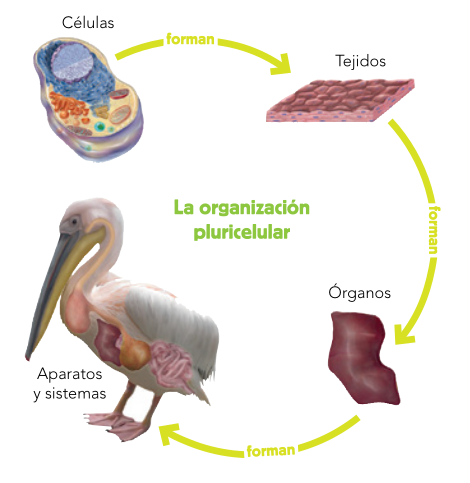
\includegraphics[width=0.5\linewidth]{Tema1/08_Organizacion_pluricelular.png}
    \caption{Organización pluricelular}
    \label{fig:organizacion-pluricelular}
\end{figure}

\begin{itemize}
    \item Los tejidos son agrupaciones de células especializadas en realizar una misma tarea. Por ejemplo, algunos seres vivos tienen tejidos, como el muscular, formado por células especializadas en producir movimientos.
    \item Los órganos son agrupaciones de tejidos que realizan tareas muy especializadas y coordinadas. Por ejemplo, hay seres vivos que tienen órganos como el corazón, que se encarga de bombear la sangre por el cuerpo.
    \item Los aparatos o sistemas son conjuntos de órganos que se agrupan para llevar a cabo un proceso más complejo. Por ejemplo, algunos seres vivos tienen aparatos como el digestivo que realiza el proceso de la digestión, formado por muchos órganos.
\end{itemize}